\documentclass[a4paper,10pt]{article}

\title{Bifurcation analysis of an ocean model}
\author{Leo Sok \& Harmen Stoppels}
\date{\today}
\usepackage{amsmath,amssymb}
\usepackage{enumitem}
\usepackage{pdfpages}
\usepackage{epstopdf}
\usepackage{graphicx}
\usepackage{subcaption}
\usepackage{booktabs}
\usepackage[font={small,it}]{caption}
\usepackage{wrapfig}
\usepackage{hyperref}
\usepackage{cleveref}
\usepackage{autonum}
\def\*#1{\mathbf{#1}}

\begin{document}
  \maketitle

  \begin{figure}[b!]
  \centerline{\includegraphics[width=1.3\textwidth]{images/bifurcatie_met_plots.pdf}}
  \caption{This bifurcation diagram gives an overview of the interesting points the ocean model. We see both a pitchfork and a Hopf bifurcation point. The subplots are the streamfunctions at the given parameters.}\label{fig:bifurcation_diagram}
  \end{figure}

  %!TEX root = ../report.tex
\section{Introduction}
We consider a simplified, homogeneous, two-dimensional, wind-driven ocean model in a square basin. After non-dimensionalizing the equations and assuming a constant density $\rho$ together with incompressibility, we can formulate the problem in terms of the stream function $\psi = \psi(t, x, y).$ This formulation basically eliminates the pressure term from the Navier-Stokes equations and automatically fulfills the continuity equation. [Something something boundary conditions.] Ultimately this leads to the following PDE:
\begin{equation}\label{eq:pde}
\begin{aligned}
  \left(\frac{\partial}{\partial t} + u \frac{\partial}{\partial x} + v \frac{\partial}{\partial y}\right) \zeta + \beta \frac{\partial \psi}{\partial x} &= -\alpha \frac{\partial \tau_x}{\partial y} + \frac{1}{Re} \Delta \zeta & \text{in } [0, \infty) \times [0,1]^2, \\
  \zeta &= \Delta \psi & \text{in } [0, \infty) \times [0,1]^2, \\
  \psi = v &= 0 & \text{on } x = 0 \text{ and } x = 1, \\
  \psi = \zeta &= 0 & \text{on } y = 0 \text{ and } y = 1
\end{aligned}
\end{equation}
where $u = -\frac{\partial \psi}{\partial y}$ and $v = \frac{\partial \psi}{\partial x}$ and the wind-stress forcing is
\begin{equation}
  \tau_x(t, x, y) = \frac{- \eta}{2 \pi} \cos{2\pi y}.
 \label{eq:tau}
\end{equation}
We keep $\alpha = \beta = 1000$ fixed, and start with $Re = 16$ and $\eta = 0,$ such that the trivial solution $\psi = 0$ satisfies~\eqref{eq:pde}. Furthermore, we discretize~\eqref{eq:pde} in space using a second-order central differences scheme on a uniform $128\times128$ grid so that the PDE reduces to a system of ODEs of the form
\begin{equation}\label{eq:ode}
  M \frac{d \*u}{d t} = F(\*u, p)
\end{equation}
with the unknown $\*u \in \mathbb{R}^{2n^2}$ and $M$ the mass matrix. Here $p$ can be interpreted as a single parameter we wish to modify, for instance $Re$ or $\eta.$ The total number of unknowns is $N = 2 n^2,$ since our grid is uniform and each grid point gives an equation for both $\psi$ and $\zeta.$

\subsection{Pseudo-arclength continuation theory}
We're looking for equilibria of~\eqref{eq:ode} where $F(\*u, p) = 0.$ In particular we want to follow an equilibrium as $p$ varies. To do so, we apply the following procedure:
\begin{enumerate}
  \item Parametrize $\Gamma(s) = (\*u(s), p(s))$ with $\|\dot\Gamma(s)\| = 1.$
  \item Find a starting point $\Gamma(s_0)$, which is not a bifurcation point, such that $F(\Gamma(s_0)) = 0.$ 
  \item Compute $\dot\Gamma(s_0)$ explicitly (only once).
  \item Repeat for $k = 0, 1, \dots$ the predictor-corrector iteration for fixed $\Delta s$ until you reach a point of interest.
  \begin{description}
    \item[Predict:] Compute the guess $$\Gamma^{(k+1)} := \Gamma(s_k) + \Delta s * \dot\Gamma(s_k).$$
    \item[Correct:] Solve for fixed $\Delta s$ the equations \begin{equation}\begin{aligned}\label{eq:hoi}
      F(\Gamma(s_{k+1})) &= 0, \\
      \dot\Gamma^T(s_k)\Gamma(s_{k+1}) &= \Delta s - \dot\Gamma(s_k)^T\Gamma(s_k).
    \end{aligned}
    \end{equation}
    where $\Gamma(s_{k+1})$ is the only unknown, via a Newton-Rhapson procedure with $\Gamma^{(k+1)}$ the initial guess.
  \end{description}
\end{enumerate}
In our case we have in step 2 the trivial solution at our disposal, but this requires that $\eta = 0$ initially. Step 3 is more involved: since $F(\Gamma(s)) = 0$ for all $s$ per definition, we differentiate with respect to $s$ and using the chain rule we find after evaluation in $s_0$
\begin{equation}\label{eqn:null}
  \begin{bmatrix}
    DF_u(s_0) & DF_p(s_0)
  \end{bmatrix}\Dot\Gamma(s_0)
  = 0 \quad \text{ and } \quad \|\dot\Gamma(s_0)\| = 1
\end{equation}
where $DF_z$ denotes the Jacobion matrix of $F$ with respect to $z.$ Equation~\eqref{eqn:null} means $\dot\Gamma(s_0)$ is a unit vector in the null space of the $N \times (N + 1)$ dimensional matrix $$D := \begin{bmatrix} DF_u(s_0) & DF_p(s_0) \end{bmatrix}.$$ Under the assumption that $\Gamma(s_0)$ is not a bifurcation point, this matrix $D$ has full rank, so the null space is indeed one-dimensional and hence \eqref{eqn:null} has a unique solution. Computing the null space can be performed by bringing $D$ into row-echelon form as $\tilde{D}$ and solving the $(N + 1) \times (N + 1)$ augmented linear system of equations
\begin{equation}
  \begin{bmatrix}
    \tilde{D} \\ e_{N+1}^T
  \end{bmatrix}
  \dot\Gamma(s_0)
  =
  e_{N}
\end{equation}
where $e_{i}$ is the $i$th standard basis vector of length $i.$ 

Lastly, we refer to the the lecture notes for the technical details of step 4, yet we will show how Equation~\eqref{eq:hoi} is obtained. Rather than requiring exactly $\|\dot\Gamma(s)\| = 1$ in the correction phase, we require only
\begin{equation}
  \|\dot\Gamma(s_k)\| \approx \dot\Gamma(s_k)^T \frac{\Gamma(s_{k+1}) - \Gamma(s_k)}{\Delta s} = 1
\end{equation}
which explains the wording {\em pseudo}-arclength. After rewriting this, it can be seen to be equivalent to the second equation of~\eqref{eq:hoi}.

  % %!TEX root = ../report.tex

% \begin{landscape}
% \thispagestyle{empty}
% \begin{figure}
% \centerline{\includegraphics[width=0.9\textwidth]{images/bifurcatie_met_plots.pdf}}
% \caption{Bifurcation diagram}
% \end{figure}
% \end{landscape}


  %!TEX root = ../report.tex
\section{Spinup}

Starting from $\eta = 0$ with the trivial solution satisfying equation~\eqref{eq:pde}, we apply continuation in $\eta$ from $0$ to $1$ in steps of $\Delta s = 0.1$ and find a non-trivial solution at $Re = 16$ as shown in Figures~\ref{fig:question_a_psi} and~\ref{fig:question_a_zeta}.

\begin{figure}[h!]
    \centering
    
    \centerline{
    \begin{subfigure}[b]{0.6\textwidth}
        \includegraphics[width=\textwidth]{images/a_psi.eps}
        \caption{Streamfunction $\psi$ at $Re = 16$.}
        \label{fig:question_a_psi}
    \end{subfigure}
    ~
    \begin{subfigure}[b]{0.6\textwidth}
        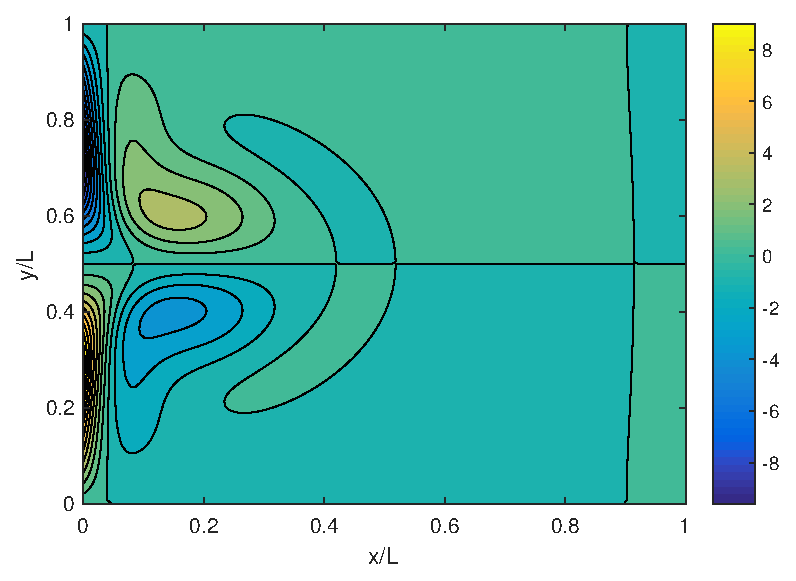
\includegraphics[width=\textwidth]{images/a_zeta.eps}
        \caption{$\zeta$ at $Re = 16$.}
        \label{fig:question_a_zeta}
    \end{subfigure}
    }
    \caption{First non-trivial solutions after spin-up.}\label{fig:question_a}
\end{figure}

  %!TEX root = ../report.tex
\section{Preconditioning}

The iterative solver is $\textrm{CGSTAB}$ with $ILU$ as a preconditioner. The preconditioner has a single parameter $\epsilon$ which determines the drop tolerance in the incomplete decomposition. A value of $\epsilon = 0$ reduces to a full LU decomposition, which requires too much work and memory, and would make an iterative method superfluous. On the other hand, if $\epsilon = 1$ the preconditioner simply reduces to a diagonal matrix, which is cheap to apply, but maybe not as effective. Typically the optimal value for $\epsilon$ must be found experimentally. In our case it turns out $\epsilon \approx 10^{-6}$ is an optimal value in terms of CPU time spent on a single continuation step in $Re$ at $Re \approx 16$ and $\eta = 1$ (given the initial direction). See Figure~\ref{fig:optimal_epsilon} for reference.

% \begin{wrapfigure}{l}{0.25\textwidth}
\begin{figure}[h]
    \centering
    \includegraphics{images/droptol_epsilon.pdf}
    \caption{Finding the optimal drop tolerance paramter $\epsilon$ experimentally.}
    \label{fig:optimal_epsilon}
\end{figure}
% \end{wrapfigure}

  \section{opgave c}

\begin{figure}
  \caption{A picture of a gull.}
  \centering
    \includegraphics[width=0.5\textwidth]{fig3d.eps}
\end{figure}

  \section{Internal symmetry}
When we use the eigenvalue solver (JDQZ) to find the value of the Reynolds number at the first pitchfork bifurcation, we find $Re_p=29.5112$

In this section, we will show the internal symmetry of the system (equation \ref{eq:pde}). What we will show is that if we have a steady state $\psi(x,y)$, then $-\psi(x,1-y)$ is also a steady state. The continuation start at Re=16 with an antisymmetric solution, so $\psi(x,y)=-\psi(x,1-y)$. After the pitchfork bifurcation, we get another solution, which is no longer antisymmetric. Thus its antisymmetric counterpart becomes also a solution, which gives us two new solutions. From this, we conclude that this bifurcation must be a pitchfork bifurcation.
 
 We now first show that if we have a steady state $\psi(x,y)$, then $-\psi(x,1-y)$ is also a steady state.
 
Suppose we have found a steady state $\psi(x,y)$ (we dropped the index $t$, because the steady state does not depend on $t$). Then, if we rewrite the PDE \ref{eq:pde}, we get
 \begin{equation}
   \frac{\partial}{\partial t}\zeta= - \underbrace{   u \frac{\partial\zeta}{\partial x}}_{=:\ref{eq:steady} a} +\underbrace{  v \frac{\partial\zeta}{\partial y}}_{=:\ref{eq:steady}b} - \beta \underbrace{\frac{\partial \psi}{\partial x} }_{=:\ref{eq:steady}c} - \alpha\underbrace{ \frac{\partial \tau_x}{\partial y}}_{=:\ref{eq:steady} d} +\frac{1}{Re}  \underbrace{\Delta \zeta}_{=:\ref{eq:steady}e}=0\label{eq:steady}
\end{equation}
 $$\zeta=\Delta \psi $$
For this $\psi(x,y)$.

Now we want to show that 
$$\bar{\psi}(x,y)=-\psi(x,\bar{y}) \text{ with }\bar{y}=1-y$$
is also a steady state.

So we want to show that, if equation \ref{eq:steady} holds, 
 \begin{equation} \frac{\partial}{\partial t}\bar{\zeta}=- \underbrace{  \bar u \frac{\partial\bar{\zeta}}{\partial x}}_{=:\ref{eq:othersteady} a} +\underbrace{ \bar v \frac{\partial\bar{\zeta}}{\partial y}}_{=:\ref{eq:othersteady}b} -\beta \underbrace{ \frac{\partial \bar{\psi}}{\partial x} }_{=:\ref{eq:othersteady}c} -\alpha  \underbrace{\frac{\partial \bar \tau_x}{\partial y}}_{=:\ref{eq:othersteady}d} + \frac{1}{Re} \underbrace{\Delta \bar{\zeta}}_{=:\ref{eq:othersteady}e}=0 \label{eq:othersteady}
 \end{equation}
 $$\bar{\zeta}=\Delta \bar{\psi}$$ 
We will show this by showing that the parts (a, b, c, d, e) in equation \ref{eq:othersteady} are minus the same part in equation \ref{eq:steady}. Therefore we will first show that $-\bar{u}=-u$ and $\bar{v}=v$. 
 
\begin{equation}
-\bar u=\frac{\partial \bar{\psi}}{\partial y}(x,y)=-\frac{\partial \psi}{\partial \bar y}(x,\bar y)\frac{\partial \bar{y}}{\partial y}=\frac{\partial \psi}{\partial \bar y}(x,\bar y)=-u
\label{eq:ubar}
\end{equation}

\begin{equation}
\bar v=\frac{\partial \bar{\psi}}{\partial x}(x,y)=-\frac{\partial \psi}{\partial x}(x,\bar y)=-v \label{eq:vbar}
\end{equation}

Before the further computations we will show that $\bar{\zeta}=-\zeta$.

\begin{align}
\bar{\zeta}(x,y) &= \Delta \bar{\psi}(x,y)
=\frac{\partial^2\bar{\psi}}{\partial x^2}(x, y)+\frac{\partial^2\bar{\psi}}{\partial \bar y^2}(x, y) \nonumber \\
&=-\frac{\partial^2\psi}{\partial x^2}(x,\bar y)-\frac{\partial^2\psi}{\partial \bar y^2}(x,\bar y)
=-\zeta(x,\bar y)\label{eq:zetabar}
\end{align}

With these, we will now show that equation \ref{eq:othersteady} follows from equation \ref{eq:steady}.
We start with part a of the equations. Using equations \ref{eq:ubar} and \ref{eq:zetabar},
\begin{equation*}
\ref{eq:othersteady} a=\bar u\frac{\partial\bar{\zeta}}{\partial x} (x,y) =-u \frac{\partial\zeta}{\partial x} (x,\bar y)=-\ref{eq:steady}a
\end{equation*}
Then part b, using equations \ref{eq:vbar} and \ref{eq:zetabar},
\begin{equation*}
\ref{eq:othersteady}b=\bar{v}\frac{\partial\bar{\zeta}}{\partial y} (x,y) =-v \frac{\partial\zeta}{\partial \bar y} (x,\bar y)=-\ref{eq:steady}b
\end{equation*}
Equality of the parts c follows immediately from equation \ref{eq:vbar}
$$\ref{eq:othersteady}c=\frac{\partial \bar{\psi}}{\partial x}=\bar{v}=-v=-\frac{\partial \psi}{\partial x}=-\ref{eq:steady}c$$
For part d, we have defined $\bar{\tau}_x(y)=\tau_x(\bar y)$, where we have dropped the indices $t$ and $x$, because $\tau$ does not depend on them. So we get
$$\ref{eq:othersteady}d=\frac{\partial \bar \tau_x}{\partial y}(y)=\frac{\partial \tau_x}{\partial \bar y}(\bar y)\frac{\partial y}{\partial \bar y}=-\frac{\partial \tau_x}{\partial \bar y}(\bar y)=-\ref{eq:steady}d$$
Finally we look at part e of the equations. Using equation \ref{eq:zetabar}, we get
\begin{align*}
\ref{eq:othersteady}e& =\Delta \bar{\zeta}(x,y)
=\frac{\partial^2\bar{\zeta}}{\partial x^2}(x, y)+\frac{\partial^2\bar{\zeta}}{\partial \bar y^2}(x, y) \\
&=-\frac{\partial^2\zeta}{\partial x^2}(x,\bar y)-\frac{\partial^2\zeta}{\partial \bar y^2}(x,\bar y)=-\Delta\zeta(x,\bar y)=-\ref{eq:steady} e
\end{align*}

Combining this five parts of equations \ref{eq:othersteady} and \ref{eq:steady} shows us that
$$\frac{\partial}{\partial t}\bar{\zeta}=-\frac{\partial}{\partial t}\zeta=0$$ and thus is $\bar{\psi}$ a steady state, which gives us the internal symmetry of the system that gives rise to the pitchfork bifurcation.




  
  %!TEX root = ../report.tex
\section{Pitchfork}


The cheapest way to continue on the stable, non-symmetric branch of the pitchfork is to break the symmetry of the PDE temporarily. This is carried out by adding a non-symmetric forcing term to the equation controlled by a new parameter {\tt asym}, continuing only a tad in the new parameter, subsequently continuing in $Re$ past the pitchfork bifurcation point, and lastly restoring symmetry by bringing {\tt asym} back to 0. To be more precise, we replace the wind stress forcing term $\tau_x$ by
\begin{equation}
    \tau_x := -\eta \left( \frac{1 - \mathtt{asym}}{2 \pi} \cos(2\pi y) + \frac{\mathtt{asym}}{\pi} \cos(\pi y) \right)
\end{equation}
such that the corresponding term in the right-hand side of the PDE~\eqref{eq:pde} becomes
\begin{equation}
    -\frac{\partial \tau_x}{\partial y} = -\eta (1 - \mathtt{asym})\sin(2\pi y) + \mathtt{asym}\sin(\pi y)).
\end{equation}
This clearly breaks the anti-symmetry $\partial_y \tau_x(y) \neq -\partial_y \tau_x(1 - y).$ We add the parameter $\mathtt{asym}$ at $Re = 16$ and continue in $\mathtt{asym}$ for two steps of $\Delta s = 0.1.$ We then continue in $Re$ until $Re \approx 31.$ At this point it becomes clear we have passed the pitchfork bifurcation point, by judging the behaviour of the solution as shown in Figure~\ref{fig:pitch_detection}. If we look at $\psi_{max}$ as a function of $Re,$ we see interesting behaviour around $Re \approx 29,$ where it suddenly increases and then flattens. Also the effective step size in $Re$ decreases while $\Delta s$ is kept constant at $0.1$; this could mean that the solution changes more rapidly. Even more pronounced is the graph of $\psi_{max} + \psi_{min}$ where we not only see the small disturbance in symmetry around $Re = 16,$ but as well how it blows up past $Re = 29.$ Another way to detect the bifurcation point is to look at a specific point of the solution such as $\psi(\tfrac{1}{8}, \tfrac{1}{8})$ or $\psi(\tfrac{3}{8}, \tfrac{3}{8})$ where a qualitative change in behaviour appears after $Re = 29.$

At $Re \approx 31$, we bring back $\texttt{asym}$ to $0.$ Next we continue to $Re = 40$ at which point we obtain the solution as plotted in Figure~\ref{fig:question_e}.

\begin{figure}[h!]
    \centering
    \caption{Detection of the pitchfork.}
    \label{fig:pitch_detection}
    \centerline{\includegraphics[width=1\textwidth]{images/pitch_detection.pdf}}
\end{figure}

\begin{figure}[h]
    \centering
    \caption{Solutions on the upper branch of the pitchfork}\label{fig:question_e}
    \centerline{
    \begin{subfigure}[b]{0.6\textwidth}
        \includegraphics[width=\textwidth]{images/e_psi.eps}
        \caption{Streamfunction $\psi$ at $Re = 40$}
        \label{fig:question_e_psi}
    \end{subfigure}
    ~
    \begin{subfigure}[b]{0.6\textwidth}
        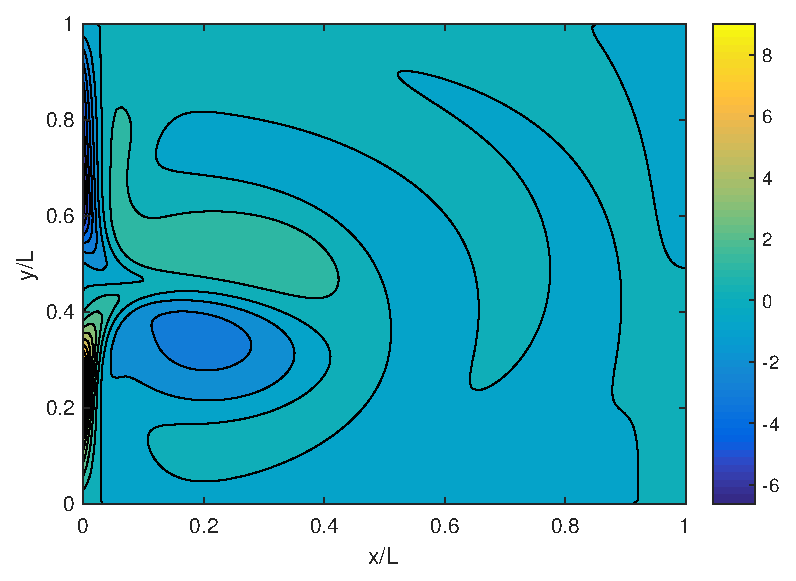
\includegraphics[width=\textwidth]{images/e_zeta.eps}
        \caption{$\zeta$ at $Re = 40$}
        \label{fig:question_e_zeta}
    \end{subfigure}
    }
\end{figure}

Now that we are on asymmetric branch of the pitchfork, we can easily get on its anti-symmetric counterpart by continuing backwards in $Re$ from $Re = 40$ to $Re_p$ and then all the way to $Re = 40$ again. This is done by setting $\Delta s = -1.$ We plot the solution in Figure~\ref{fig:question_e_lower}.

\begin{figure}[h]
    \centering
    \caption{Solutions on the lower branch of the pitchfork}\label{fig:question_e_lower}
    \centerline{
    \begin{subfigure}[b]{0.6\textwidth}
        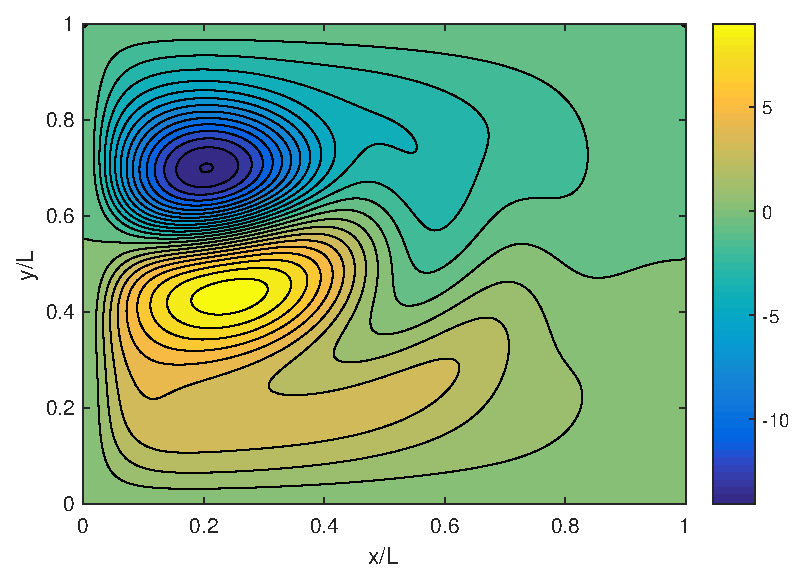
\includegraphics[width=\textwidth]{images/e_psi_lower.eps}
        \caption{Streamfunction $\psi$ at $Re = 40$}
        \label{fig:question_e_psi_lower}
    \end{subfigure}
    ~
    \begin{subfigure}[b]{0.6\textwidth}
        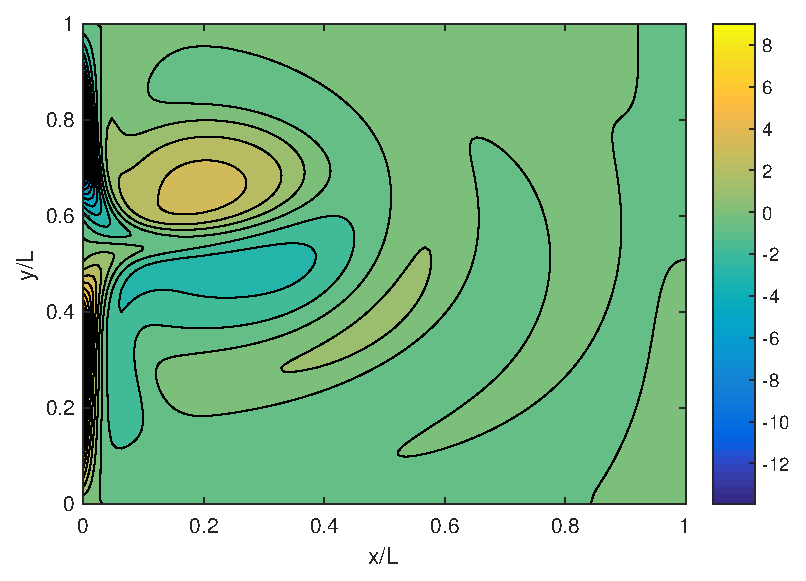
\includegraphics[width=\textwidth]{images/e_zeta_lower.eps}
        \caption{$\zeta$ at $Re = 40$}
        \label{fig:question_e_zeta_lower}
    \end{subfigure}
    }
\end{figure}

  %!TEX root = ../report.tex
\section{Hopf bifurcation}

Continuing on the upper branch of the pitchfork, we compute (at most) 6 of the eigenvalues closest to the origin after a few steps in $Re.$ After a while we find that a conjugate eigenpair crosses the imaginary axis, which indicates a Hopf bifurcation is nearby. The movement of the eigenvalues is visualized in Figure~\ref{fig:eigenpair_crossing_imag}.

\begin{figure}[h]
  \centerline{\includegraphics[width=\textwidth]{images/eigenwaarden_hopf.pdf}}
  \caption{A conjugate eigenpair crossing the imaginary axis.}
  \label{fig:eigenpair_crossing_imag}
\end{figure}

We apply the secant procedure to compute the value of $Re$ where the first eigenvalue $\lambda$ is completely imaginary, i.e. $\Re(\lambda) = 0.$ We find that the Hopf bifurcation is located at $Re_H \approx 68.9781.$ The conjugate eigenpair is $$\lambda_\pm \approx \pm 9.372i.$$

The real and imaginary part of the eigenfunctions corresponding to $\lambda_+$ is shown in Figure~\ref{fig:eigenfunction}. Note that the eigenfunction of $\lambda_-$ is identical up to a sign flip in the complex part.

\begin{figure}[h]
    \centering
    \caption{Eigenfunctions corresponding to $\lambda \approx 9.372i$.}\label{fig:eigenfunction}
    \centerline{
    \begin{subfigure}[b]{0.6\textwidth}
        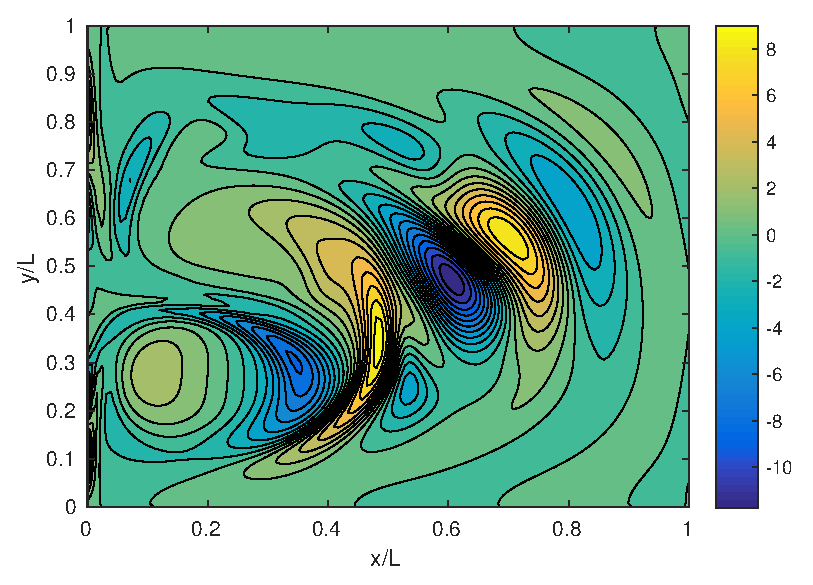
\includegraphics[width=\textwidth]{images/eigenvector_hop_1_2.eps}
        \caption{Real part corresponding to $\psi$}
        \label{fig:nm32}
    \end{subfigure}
    ~
    \begin{subfigure}[b]{0.6\textwidth}
        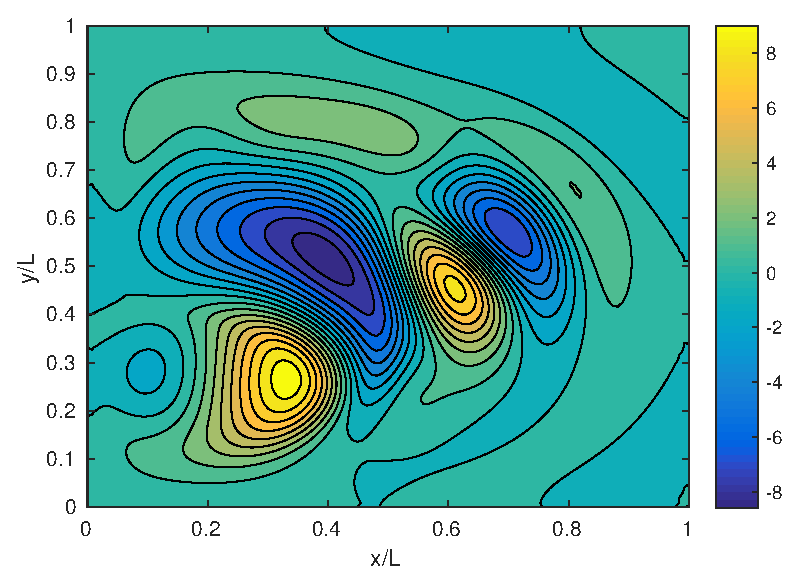
\includegraphics[width=\textwidth]{images/eigenvector_hop_2_2.eps}
        \caption{Real part corresponding to $\zeta$}
        \label{fig:nm64}
    \end{subfigure}
    }
    \centerline{
    \begin{subfigure}[b]{0.6\textwidth}
        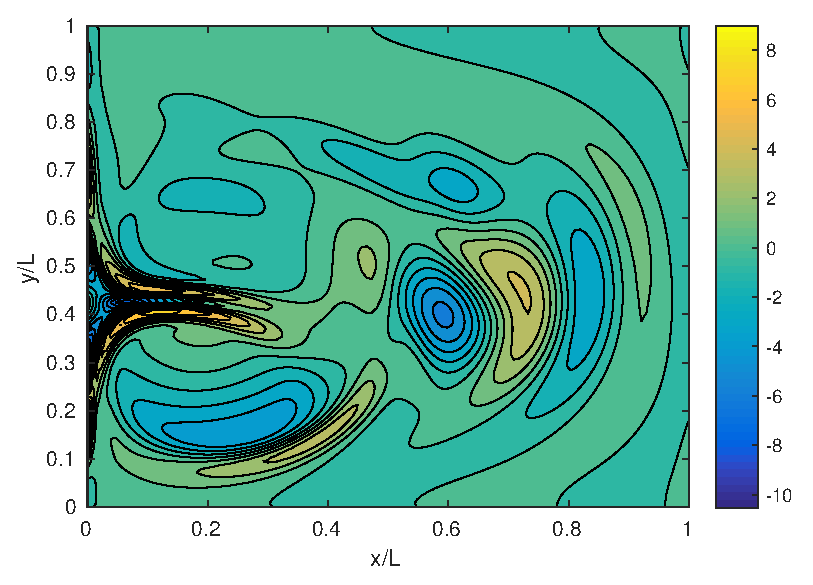
\includegraphics[width=\textwidth]{images/eigenvector_hop_1_3.eps}
        \caption{Imaginary part corresponding to $\psi$}
        \label{fig:nm32}
    \end{subfigure}
    ~
    \begin{subfigure}[b]{0.6\textwidth}
        \includegraphics[width=\textwidth]{images/eigenvector_hop_2_3.eps}
        \caption{Imaginary part corresponding to $\zeta$}
        \label{fig:nm64}
    \end{subfigure}
    }
\end{figure}
  
  \section{Conclusion}
We have looked at the steady states of the homogeneous wind-driven ocean circulation. We started with a trivial steady state with no wind-stress forcing and Reynolds number 16. From this steady state, we used a pseudo-arclength continuation in the wind forcing till we had full wind forcing. We found a steady state for which the streamfunction was symmetric. From this steady state, we applied a continuation in the Reynolds number to find a pitchfork bifurcation. This bifurcation appeared to be at $Re_p=29.5112$. In order to find the branches of asymmetric solutions, we started again at the steady state for $Re=16$. We broke the symmetry of the pitchfork by adding a non-symmetric forcing term. We applied a continuation in Re in this asymmetric system till we passed the bifurcation point. When we where at $Re\approx 31$, we went back to the original symmetric forcing system. So we and up on one of the branches of asymmetric solution. We used again the pseudo-arclength continuation, but now backwards in Re, following the branch through the bifurcation point and we found the other asymmetric branch.

After we found the pitchfork bifurcation, we also tried to find a Hopf-bifurcation. We started at the upper asymmetric branch of the pitchfork. The Hopf-bifurcation can only be detected by looking at the eigenvalues. So we applied a continuation in Re again, but at each step, we computed the eigenvalues and found that at $Re_H=68.9781$ a conjugate eigenpair crosses the imaginary axis and thus is there a Hopf bifurcation.
\end{document}